\documentclass{llncs}
%\usepackage{amsmath,amsthm,amssymb,fullpage,yfonts,graphicx,proof,subfig,wrapfig,appendix,hyperref,mdwlist,wasysym}
%\usepackage{amsmath,amsthm,amssymb,fullpage,yfonts,graphicx,proof,appendix,hyperref,mdwlist,wasysym}
\usepackage{amsmath,amssymb,fullpage,yfonts,graphicx,proof,appendix,hyperref,mdwlist,wasysym}
\usepackage{upgreek}
%\usepackage{times}
%\usepackage[charter]{mathdesign}
\usepackage{hyperref}
\usepackage{algorithm}
\usepackage{algpseudocode}
\usepackage{multirow}
\usepackage[usenames,dvipsnames]{xcolor}
%\usepackage{epsfig}
\usepackage[bottom]{footmisc}
%\usepackage{mjz-titlepage}
\usepackage{framed}
\usepackage{setspace}
\setstretch{1.05}
\usepackage{subfig}
\usepackage{changebar}
\usepackage{colortbl}
\usepackage{wrapfig}

\begin{document}
%\captionsetup{width=.75\textwidth,font=small,labelfont=bf}

%%%%%%%%%%%%%%%%%%%%%%%%
\title{\bf Landslide: \\ Systematic Exploration for Kernel-Space Race Detection}
\author{Ben Blum \and Garth Gibson}
\institute{Computer Science Department, Carnegie Mellon University, Pittsburgh, PA}
\date{May 2012}

\maketitle

%%%%%%%%%%%%%%%%%%%%%%%%
\newcommand\true{\;\textit{true}}
\newcommand\false{\;\textit{false}}

\newcommand\alpher\alpha
\newcommand\beter\beta
\newcommand\gammer\gamma
\newcommand\delter\delta
\newcommand\zeter\zeta
\newcommand\Sigmer\Sigma

\newcommand\NN{\mathbb{N}}
\newcommand\QQ{\mathbb{Q}}
\newcommand\RR{\mathbb{R}}
\newcommand\ZZ{\mathbb{Z}}

\setcounter{changebargrey}{35}
%\newcommand\revision[1]{\begin{samepage}\cbstart#1\cbend\end{samepage}}
%\newcommand\revision[1]{\cbstart#1\cbend}
\newcommand\revision[1]{#1}

\begin{abstract}
Systematic exploration is an approach to finding race conditions by deterministically executing many thread interleavings and identifying which ones expose bugs.
Current techniques are suitable for testing user-space programs, but are inadequate for testing operating system kernels.
Testing kernel-level code necessitates understanding the kernel's design in order to effectively control nondeterminism and achieve reasonable state-space reduction.
% paragraph split would go here, but abstrax
We present Landslide, a systematic exploration tool for finding races in kernels.
Landslide makes use of user-provided configuration to enable efficient exploration and testing of meaningful interleavings.
The user instruments the kernel to inform Landslide of important concurrency events, and configures Landslide's search to de-emphasize irrelevant kernel components.
This combines the user's design knowledge with Landslide's ability to explore large state spaces.
Our experience with Landslide shows that a tool built for this usage pattern is capable of identifying otherwise-overlooked kernel-space races.

%, and encourages the user to steer Landslide towards focused searches that are more likely to find bugs.
%We claim that this steering is an effective approach for kernel-space race detection.

%Landslide targets Pebbles, the kernel specification that students implement in the undergraduate Operating Systems course at Carnegie Mellon University (15-410).
%We discuss the techniques Landslide uses to address the general challenges of kernel-level concurrency, and we evaluate its effectiveness and usability as a debugging aid.
%We show that our techniques make systematic testing in kernel-space feasible and that Landslide is a useful tool for doing so in the context of 15-410.
%%%%

\noindent {\bf Keywords:} concurrency, kernel debugging, race conditions, runtime verification
\end{abstract}

%%%% Outline %%%%

% challenges of kernel space
% = causes of concurrency
% = ad-hoc
% - design independence (merge into model/scope)
%
% implementation
% + model (maybe separate into a scope section, add talk of 15410)
% - components (keep only challenge-addressing stuff)
% + bug identification
% = por (-soundness)
%
% user interface
% - requirements (timer-driven should be in model)
% = instrumenting (cut very short)
% + configuring
% = test cases (merge into model maybe -- probably not though?)
%
% future work
% - education
% = new techniques
% + linux
% = virtualisation (merge into linux?)
% ? shaping
% - oddities

%%%%% better outline %%%%
% intro
% related
% challenges of kernel-space (short section, 2-3 paragraphs)
% - causes of concurrency
% - ad-hoc memory sharing
% scope and model
% - summary of 410 & kernel requirements
% - simulated execution
% - timer-driven scheduling/concurrency
% - orientation for false-negative bugs & coarse-granularity search
% implementation
% - components (very briefly; only keep challenge-solving stuff)
% - bug identification techniques
% - making DPOR work
% user interface
% - instrumenting process
% - iterative configuring + focusing of search
% - types of test cases to use
% future work
% - new techniques to incorporate
% - virtualisation and linux
% - maybe shaping? (not sure how i could say it quickly.)


% \newcommand\squish{\vspace{-8pt}}
\newcommand\squish{}

%%%%%%%%%%%%%%%%%%%%%%%%%%%%%%%%%%%%%%%%%%%%%%%%%%%%%%%%%%%%%%%%%%%%%%%%%%%%%%%%
\squish
\section{Introduction}
\squish
%%%%%%%%%%%%%%%%%%%%%%%%%%%%%%%%%%%%%%%%%%%%%%%%%%%%%%%%%%%%%%%%%%%%%%%%%%%%%%%%

Race conditions are notoriously difficult to debug.
Because of their nondeterministic nature, they frequently do not manifest at all during testing, and when they do manifest, it is difficult to reproduce them reliably enough to collect enough information to help debugging.

Systematic exploration~\cite{verisoft} is a dynamic testing technique that aims to find race conditions. It involves enumerating many different interleavings of multiple threads and forcing a system to execute all such interleavings to check if any expose bugs.
% In comparison with conventional stress testing, systematic exploration is less likely to overlook bugs, due to its deterministic testing approach.
While other dynamic analysis techniques exist for finding race conditions, such as data race detection \cite{datacollider},
systematic exploration is able to find a wider range of types of concurrency errors because of its ability to manipulate the execution of the system under test.

%\revision{
%Many techniques exist for dynamic testing of concurrent systems for race conditions.
%Systematic exploration~\cite{verisoft}, the strategy we focus on in this work, involves making educated guesses as to what points during execution a preemption would be most likely to expose a bug, enumerating the different possibilities for interleaving threads around these points, and forcing the system to execute all such interleavings to check if any of them results in incorrect behaviour.
%Systematic exploration provides a better alternative to conventional long-running stress tests, because it is less likely to overlook buggy execution patterns, and it enables a testing framework to report more thorough debugging information. Compared to other dynamic analyses, such as data race detection~\cite{datacollider}, systematic exploration is able to find a wider range of types of concurrency errors because of its ability to manipulate the execution of the system under test.

In kernel space, race condition debugging becomes even more difficult. Many aspects of the concurrency implementation itself are part of the system being tested.
While user-space testing frameworks operate above clear abstractions and interfaces, a systematic exporation tool for kernels cannot rely on such easy means of understanding the system under test.
Furthermore, execution in the scheduler and in similar components is common to all concurrent threads, even otherwise independent ones; this threatens our ability to achieve state-space reduction.

%While user-space testing frameworks rely on the underlying kernel to provide common concurrency abstractions which the framework can use to drive the test, systematic exploration in the kernel itself necessarily exists underneath such abstractions.
%Furthermore, a tool that supports testing multiple kernels must support many different possible scheduler designs.

% The claim of this dissertation is as follows.
% \begin{quote}
% \bf
% Systematic exploration in kernel space is possible by understanding a kernel's concurrency through instrumentation of its internal abstractions, and can be made efficient by relying on the user to control the scope of the test.
% \end{quote}
% }

We present Landslide \cite{landslide},
%\footnote{Landslide {\em (n)}: a phenomenon which demonstrates that Pebbles are not as stable as you might think.}
a tool for applying systematic race detection techniques to kernel-level code.
Landslide is implemented as a module for Wind River Simics\textsuperscript{\texttrademark}~\cite{simics}, and targets Pebbles \cite{kspec}, a fully preemptible UNIX-like kernel specification that students implement in Carnegie Mellon University's senior level operating systems class (15-410).
% To use Landslide efficiently, a programmer must instrument their kernel to inform Landslide of important concurrency events. In order to make Landslide's search efficient, the programmer should also configure Landslide to focus on the most relevant parts of the test at hand.
Landslide's interface allows the user to configure its search to focus on the most relevant parts of the test at hand, which leads to a usage dynamic that combines the user's design knowledge and Landslide's exploration mechanisms. Intuitively, the user ``steers'' Landslide towards search spaces that are more likely to quickly find suspected bugs.

%It is geared towards kernels that implement the Pebbles specification, the main project in Operating System Design and Implementation (15-410) at CMU, and is implemented as a module for Wind River Simics\textsuperscript{\texttrademark}~\cite{simics}, the x86 simulator that students use to run their Pebbles kernels.
%\revision{In order to use Landslide, a kernel programmer must instrument their kernel to inform Landslide of important concurrency events during the execution, and configure Landslide to focus its search on components of the kernel most relevant to the test.
%During a kernel's execution, Landslide records important actions performed by the kernel, decides at which points in the kernel's execution a preemption will be most likely to expose a bug, and then exercises all possible interleavings of kernel threads around such points.
%Using this instrumentation and configuration, Landslide is able to enumerate all possible interleavings of kernel threads at a granularity both fine-grained enough to expose interesting concurrency behaviour and coarse-grained enough to produce state spaces that are feasible to explore. Landslide then forces the kernel to exercise each of these interleavings, and checks for race conditions in each of them.}
%When Landslide finds a bug (predicted by a set of common checks and heuristics), it stops execution and prints information about the sequence of interleavings that exposed the bug.

We found that, with modest instrumentation effort, Landslide was able to find race conditions in several different Pebbles kernels. These races had previously been overlooked by stress testing and/or expert manual inspection.
Many of these bugs required complicated thread interleavings to expose, and could not have been found with simpler testing techniques such as data race detection or static analysis.
% TODO: decide whether to prove it?

%\revision{
%In this work, we study the challenges inherent in applying systematic testing techniques in kernel-space, in contrast with user-space applications (Chapter~\ref{sec:challenges}), define common terms used in the rest of this document (Chapter~\ref{sec:terminology}), present our techniques (some sound, and some heuristic) for addressing them (Chapter~\ref{sec:design}), and document the process of using Landslide (Chapter~\ref{sec:using}).
%We evaluate Landslide both by studying its potential to be a helpful debugging aid in 15-410 and by studying certain bugs in detail to determine effective usage strategies (Chapter~\ref{sec:evaluation}).
%Finally, we discuss possible avenues for future work in education, use of additional testing techniques, application to general purpose kernels, long-running testing approaches, and theoretical study of systematic exploration (Chapter~\ref{sec:future}).
%}

%%%%%%%%%%%%%%%%%%%%%%%%%%%%%%%%%%%%%%%%%%%%%%%%%%%%%%%%%%%%%%%%%%%%%%%%%%%%%%%%
\squish
\section{Related Work}
\squish
%%%%%%%%%%%%%%%%%%%%%%%%%%%%%%%%%%%%%%%%%%%%%%%%%%%%%%%%%%%%%%%%%%%%%%%%%%%%%%%%

Among related dynamic race condition detection tools, some are systematic exploration tools, and others are kernel race-finding tools. To our knowledge, Landslide is the first to combine the former with the latter.

{\bf Systematic exploration.} Many techniques have been developed for efficient systematic exploration of concurrent systems. Dynamic Partial Order Reduction (DPOR) \cite{dpor} is an algorithm for achieving state space reduction by identifying ``independent'' thread transitions. dBug \cite{dbug-ssv} is a user-space tool that uses DPOR in user-space; Landslide applies it to test kernels.

Among other user-space systematic testing tools are CHESS \cite{chess}, with a heuristic for search ordering based on number of preemptions; MaceMC \cite{macemc} and MODIST \cite{modist}, which test networked and distributed applications; RacePRO \cite{racepro}, which uncovers inter-process races around system call invocations; and DeMeter \cite{demeter}, which focuses its search on only one component of a system at a time.

{\bf Kernel-level verification.}
% Kernel-level code has seen many dynamic testing techniques apart from systematic exploration.
DataCollider \cite{datacollider} uses memory access sampling to find data races in Windows 7. Compared to systematic exploration, data race detection is less expensive, but is limited in which types of races it can find.
% Carburizer \cite{carburizer} is a tool for enhancing resiliency of imperfect kernel drivers in the presence of faulty peripheral devices.
SimTester \cite{simtester} is a tool for testing kernel drivers; like Landslide, it runs in Simics, and injects interrupts to control the system's concurrency. SimTester focuses on races involving device interrupts, whereas Landslide focuses on non-driver inter-thread races. Additionally, SimTester injects only one interrupt per test run, which is less expensive than systematic exploration, but less powerful as well.

%%%%%%%%%%%%%%%%%%%%%%%%%%%%%%%%%%%%%%%%%%%%%%%%%%%%%%%%%%%%%%%%%%%%%%%%%%%%%%%%
\squish
\section{Scope}
\squish
%%%%%%%%%%%%%%%%%%%%%%%%%%%%%%%%%%%%%%%%%%%%%%%%%%%%%%%%%%%%%%%%%%%%%%%%%%%%%%%%
% \subsection{Environment}
% 410, requirements, simulated

% Landslide's ability to test different types of kernels in different execution environments is currently very limited.
% We built Landslide to test Pebbles kernels, which students implement from the ground up in a six-week project in 15-410 at CMU.

To constrain the problem space some, we aimed to use a less complex kernel than production kernels such as Linux or Windows. We built Landslide to test Pebbles kernels, which students at CMU develop from scratch in a 6 week project. These kernels are necessarily less complex, yet still rife with race conditions that are debugged furiously every semester.
The Pebbles specification \cite{kspec} is a set of UNIX-like system calls which includes routines for thread lifecycle management and virtual memory management. Among these are \texttt{fork} and \texttt{exec}, \texttt{exit} (known as \texttt{vanish}) and \texttt{wait}, and \texttt{yield}.

{\bf Testing environment.} Landslide is implemented as a module for Simics, a full-system x86 simulator which students in 15-410 use as an execution environment for their kernels. Simics can load Landslide while booting a kernel, and calls into Landslide once per instruction and once per memory access of the simulated execution. Landslide will then perform systematic exploration on that kernel using Simics interface calls to control the kernel's execution.

Landslide assumes that timer interrupts are the only nondeterministic events that influence a kernel's concurrent execution. While this prevents us from finding races related to external input such as disk or network I/O, Landslide is already able to find many types of complicated races by controlling timer-driven thread scheduling.
Landslide's model is also restricted to uniprocessor execution. Supporting multiprocessor environments, device driver testing, and production kernels is left to future work.

% \subsection{Testing Approach}

{\bf Testing approach.} Landslide's testing approach is false-negative-oriented both in terms of identifying bugs and in terms of constructing the state space to search. 
We identify bugs only when something definitely wrong happens, rather than flagging suspicious behaviours which might indicate underlying bugs, and we allow the user to manually define a granularity for thread interleavings which will produce the most meaningful results.

% %%%%%%%%%%%%%%%%%%%%%%%%%%%%%%%%%%%%%%%%%%%%%%%%%%%%%%%%%%%%%%%%%%%%%%%%%%%%%%%%
% \section{Challenges of Kernel Space}
% %%%%%%%%%%%%%%%%%%%%%%%%%%%%%%%%%%%%%%%%%%%%%%%%%%%%%%%%%%%%%%%%%%%%%%%%%%%%%%%%
% FIXME: maybe say in each paragraph how we address the issue?

% Compared to systematic exploration in user space, Landslide faces several challenges when applying the same techniques in kernel space.

% {\bf Causes of concurrency.} In user space, a testing framework may rely on system calls to the underlying kernel to deterministically control the concurrent execution of the system under test.
% However, since Landslide tests the kernel itself, it must control the underlying causes of nondeterminism, such as interrupts from the timer, disk, or network. (In this work we focus only on timer events, as discussed in \S\ref{sec:environment}.)
% Landslide contains its own internal scheduler, which manages timer interrupts to provide a mechanism for causing an arbitrarily-chosen thread to preempt execution of the current one (see \S\ref{sec:design}).

% {\bf Understanding the kernel's design.} In order to track the state of the kernel's scheduler, such as which threads exist or are runnable at any given time, a testing framework must know when certain important concurrency events happen during the kernel's execution.
% Landslide relies on in-kernel annotations to provide this information (see \S\ref{sec:instrument}).


%%%%%%%%%%%%%%%%%%%%%%%%%%%%%%%%%%%%%%%%%%%%%%%%%%%%%%%%%%%%%%%%%%%%%%%%%%%%%%%%
\squish
\section{Design}
\squish
%%%%%%%%%%%%%%%%%%%%%%%%%%%%%%%%%%%%%%%%%%%%%%%%%%%%%%%%%%%%%%%%%%%%%%%%%%%%%%%%
\label{sec:design}
% prelude: define decision point and maybe voluntary reschedule

The driving concept of Landslide's exploration is the idea of {\em decision points}. These are places in the kernel under test at which we force preemptions and around which we cause different threads to interleave. Searching with few decision points results in coarser-grained interleavings, shorter test execution, and less likelihood of finding bugs; searching with more results in the opposite.

Landslide automatically identifies a minimal set of decision points at voluntary reschedules between threads (e.g. \texttt{yield}). We provide an interface for configuring additional decision points, described in \S\ref{sec:config}.

\squish
\subsection{Exploration Mechanism}
\squish

Landslide's exploration mechanism has two parts. First, at each decision point, it can force an arbitary thread to run in place of the current one. Second, upon termination of the test case, it reverts the system to an earlier state to explore additional interleavings.

{\bf Thread scheduling.} Compared with user-space testing frameworks, Landslide cannot rely on kernel-provided system calls to control the concurrent execution of the system under test. Instead, Landslide has an internal abstraction for scheduling arbitrary threads built upon injecting timer interrupts.
If thread $M$ is running and Landslide decides to preempt with thread $N$, it fires a timer interrupt and waits for the kernel to finish the triggered context switch. Then if the kernel is running a thread that is not $N$, Landslide repeats until thread $N$ begins running, at which point it lets the kernel continue execution.

In order to know which threads are runnable at each decision point, Landslide maintains a mirror image of the kernel's scheduler state. This consists of a runqueue (all immediately runnable threads), a sleep queue (all threads blocked on \texttt{sleep} -- we treat these as runnable, because a finite number of timer ticks can cause these to run), and a descheduled queue (all other existing threads).
Landslide uses the user-provided scheduler annotations (described in \S\ref{sec:instrument}) to keep this mirror image up-to-date.

{\bf Backtracking.} Landslide makes use of Simics ``bookmarks'', a feature
which enables checkpointing and restoring the kernel's execution state, to implement
backtracking when the end of the test case is reached.

\squish
\subsection{Identifying Bugs}
\squish

%\begin{wrapfigure}{r}{0.2\textwidth}
%	\center
%	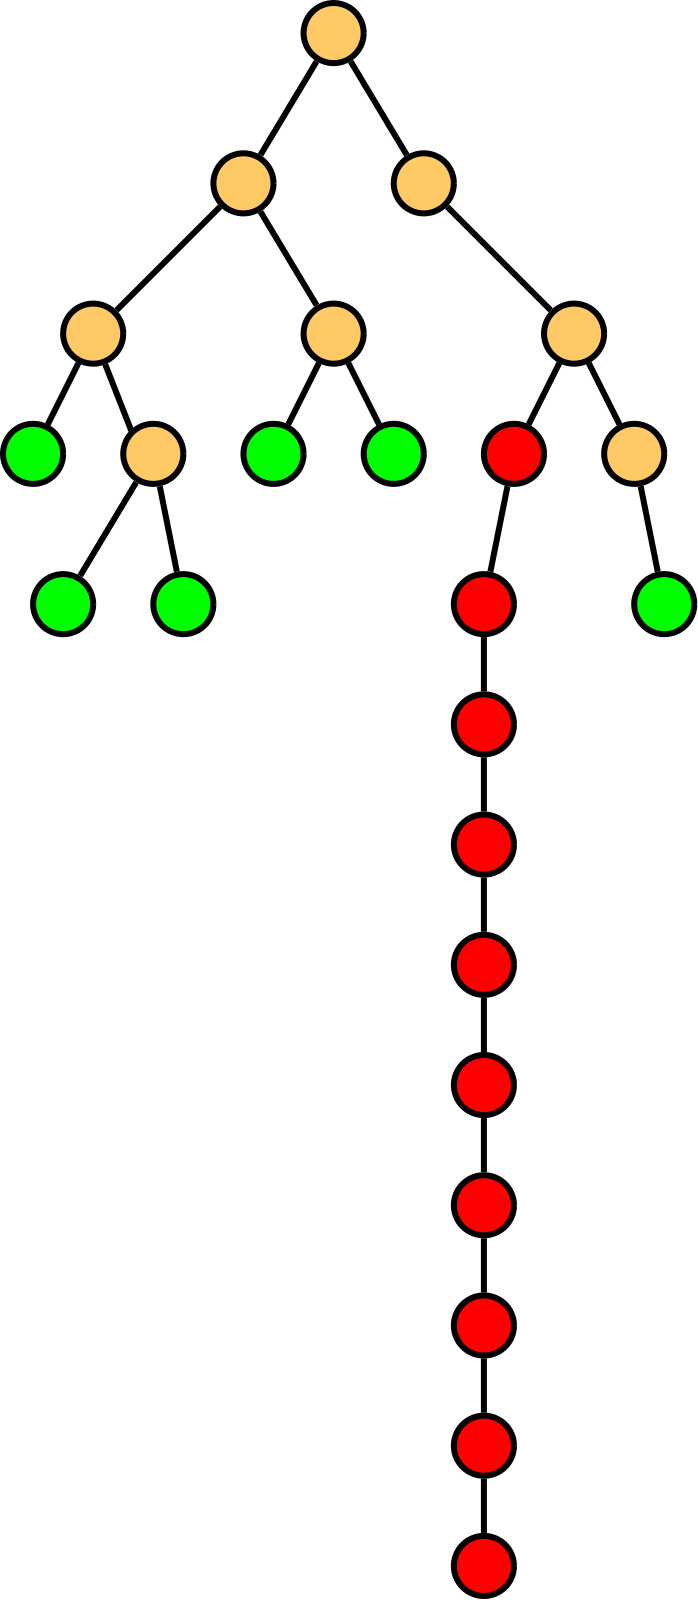
\includegraphics[width=0.2\textwidth]{livelock.pdf}
%	\caption{Infinite loop detection. Each circle represents a decision point; each branch represents one interleaving. Disproportionately many decision points have been encountered in the highlighted interleaving, which indicates the kernel is likely stuck.}
%\end{wrapfigure}

Landslide has several checks that detect when a bug arises. It can identify kernel panics, use-after-free accesses (and other memory errors such as double-free and memory leaks), and deadlocks.

Landslide can optionally also check heuristically for infinite loops and livelock. This is done by comparing the length of the current interleaving against previously-explored ones: if the current interleaving has been running disproportionately longer (by a large arbitrary constant factor), it indicates the kernel is likely stuck.
We have never found this technique to erroneously report bugs (false positives), although it may fail to trigger when it ought to if too few previous interleavings have been tested to make a reliable comparison.

When Landslide identifies a bug, it halts execution and generates a {\em decision trace}. This trace reports what kind of bug was detected (for uses-after-free, it also prints stack traces for when the block was allocated and freed), and also reports each decision point in the current interleaving: which thread was running, a trace of its stack when it was switched away from, and the thread that we caused to preempt it. With this information, the user can better understand the concurrent execution that led to the race.

In general, with false-negative bug detection, the kernel might execute a buggy behaviour yet Landslide would miss it. However (except in the case of heuristic infinite loop detection), when Landslide does identify a bug, the user can be sure that a race exists.

% decision trace

%\begin{figure}
%	\centering
%	{\small
%	\begin{tabular}{l}
%	\texttt{void add\_to\_runqueue(tcb\_t *thread) \{} \\
%	\texttt{~~~~tell\_landslide\_on\_rq(thread->id);} \\
%	\texttt{~~~~list\_insert(\&runqueue, thread);} \\
%	\texttt{\}} \\
%	\end{tabular}
%	}
%	\caption{Example annotated code.}
%\end{figure}

%%%%%%%%%%%%%%%%%%%%%%%%%%%%%%%%%%%%%%%%%%%%%%%%%%%%%%%%%%%%%%%%%%%%%%%%%%%%%%%%
\squish
\section{User Interface}
\squish
%%%%%%%%%%%%%%%%%%%%%%%%%%%%%%%%%%%%%%%%%%%%%%%%%%%%%%%%%%%%%%%%%%%%%%%%%%%%%%%%
\label{sec:interface}

\subsection{Instrumenting Kernels with Landslide}
\squish
\label{sec:instrument}

Users annotate their kernels to inform Landslide of certain important concurrency events during execution. We provide a set of annotation functions, called \texttt{tell\_landslide}, for this purpose. The annotations denote when a thread runs \texttt{fork}, \texttt{sleep}, or \texttt{exit}, when a thread is added to or removed from the runqueue, and when threads become blocked on mutexes.
There is also a configuration file, \texttt{config.landslide}, in which the user must specify constant information such as the function names of the timer handler and context switcher, which threads exist when the kernel boots, and which userspace test program Landslide should invoke.
Finally, there are two short (nominally two-line) functions used within Landslide itself that the user must implement. These are predicates on the kernel's scheduler state, and express potentially nontrivial conditions: whether the current thread is runnable but not on the runqueue, and whether preemption is disabled while interrupts are on.

\squish
\subsection{Configuring Landslide}
\squish
\label{sec:config}

After the user successfully instruments their kernel and explores a minimal state space, they should then configure Landslide's search to be more likely to find suspected bugs. For brevity, we omit discussion of some conceptually unimportant configuration options.

{\bf Configuring decision points.} Using only the decision points automatically identified on voluntary reschedules will result in coarse-grained interleavings likely to overlook bugs. We provide an extra annotation, \texttt{tell\_landslide\_decide()}, for the user to add more decision points for a finer-grained search. We recommend using it in concurrency primitives, such as at the start of \texttt{mutex\_lock()} and at the end of \texttt{mutex\_unlock()}. 

This strategy may cause Landslide to identify decision points in unrelated parts of the kernel, such as when accessing mutexes in unrelated system calls. We provide interface options in \texttt{config.landslide} for the user to view currently identified decision points and to selectively limit them. First, the user writes ``\texttt{DECISION\_INFO\_ONLY}'' to make Landslide run only one interleaving and then print all decision points instead of continuing to explore. Then, the user writes ``\texttt{within\_function foo}'' to whitelist function \texttt{foo}, and ``\texttt{without\_function bar}'' to blacklist function \texttt{bar}. For example, if testing thread death and reaping, the user should write \texttt{within\_function exit}, and \texttt{within\_function wait}, and perhaps \texttt{without\_function destroy\_address\_space} (if they don't care about the virtual memory operations associated with \texttt{exit}).

{\bf Configuring Dynamic Partial Order Reduction.} Performing DPOR \cite{dpor} requires establishing a memory independence relation between transitions.
Unfortunately, since the kernel contains its own concurrency implementation, every thread switch will execute through a common path that modifies shared scheduler data structures.
Unchecked, this would cause every transition to conflict with each other and result in no reduction in execution time from DPOR.
Certain other shared memory conflicts also arise that are irrelevant to whichever system calls are being tested; for example, if testing for races in thread lifecycle routines, the user likely does not care about accesses to the frame allocator mutex.

We provide an interface with which the user can configure Landslide to ignore such unrelated conflicts to more efficiently test components of the kernel they care about. In \texttt{config.landslide}, the user writes ``\texttt{ignore\_sym}'' followed by the name of the global variable to ignore and its type size, and Landslide may then identify transitions as independent even if they conflict on that memory.

%%%%%%%%%%%%%%%%%%%%%%%%%%%%%%%%%%%%%%%%%%%%%%%%%%%%%%%%%%%%%%%%%%%%%%%%%%%%%%%%
\squish
\section{Evaluation}
\squish
%%%%%%%%%%%%%%%%%%%%%%%%%%%%%%%%%%%%%%%%%%%%%%%%%%%%%%%%%%%%%%%%%%%%%%%%%%%%%%%%

We evaluated Landslide in two ways: first, by instrumenting two kernels we were familiar with to measure time spent to find different races, and second, by meeting with this year's 15-410 students before they submitted their kernel for grading to see if they could find bugs on their own with Landslide.

We instrumented one kernel written by an author in a previous year, and also one kernel the same author manually graded as a teaching assistant. We configured Landslide to search for five complicated already-known race conditions. In addition to finding all five races, Landslide also found a sixth previously unknown race in said author's own kernel. Using decision points only on calls to \texttt{mutex\_lock} and on voluntary reschedules, Landslide found each of the six bugs in 11 to 57 seconds, executing between 1 and 377 distinct interleavings for each.

In the user study of current students, we found that students spent on average 119 minutes (60 to 158) on the required instrumentation, and a further 36 minutes (10 to 60) refining Landslide's search. Of the four groups who finished the required part, all four found previously unknown bugs with Landslide: two races and two deterministic errors. These bugs manifested as infinite loops, a kernel panic, and a use-after-free.

%%%%%%%%%%%%%%%%%%%%%%%%%%%%%%%%%%%%%%%%%%%%%%%%%%%%%%%%%%%%%%%%%%%%%%%%%%%%%%%%
\squish
\section{Conclusion}
\squish
%%%%%%%%%%%%%%%%%%%%%%%%%%%%%%%%%%%%%%%%%%%%%%%%%%%%%%%%%%%%%%%%%%%%%%%%%%%%%%%%

We have built Landslide, a tool for systematic exploration on kernel-level code. Landslide runs as a Simics module during simulated execution of Pebbles kernels. It uses user-provided instrumentation to keep track of the kernel's state, such as the set of runnable threads, and it provides the user configuration options for making its search more effective. It identifies decision points in the kernel around which to interleave thread executions, and it controls how threads preempt each other by injecting timer interrupts. We found that Landslide identified previously unknown bugs in kernels we were already familiar with, and also that novice kernel programmers were able to find otherwise-overlooked bugs with Landslide without investing large amounts of time.


\bibliography{citations}{}
\bibliographystyle{splncs03}

\end{document}
